\chapter{Lỗ đen, lỗ trắng và sơ đồ nhân quả toàn cục}

\lectureoverview{Một chân trời về mặt cục bộ thì bình thường nhưng trên bình diện toàn cục lại có tính quyết định. Ta bắt đầu với metric Schwarzschild gần chân trời, lần theo nó đi ra ngoài bằng phép loại suy điếu xì gà Euclid, rồi hỏi Alice và Bob thực sự có thể nhìn thấy gì. Điểm kỳ dị và vùng lỗ trắng đảo chiều thời gian mở rộng bức tranh cục bộ đó thành không-thời gian Schwarzschild vĩnh cửu. Phép compact hóa Penrose làm cho cấu trúc nhân quả trở nên hữu hạn và dễ đọc. Bước cuối cùng chuyển từ một nghiệm vĩnh cửu sang một lỗ đen được tạo thành bởi sự suy sụp, nơi định lý vỏ cầu của Newton và định lý Birkhoff cung cấp các mảnh ghép cần được nối lại.}

\section{Từ chân trời đến vô cực}

Gần một chân trời Schwarzschild đủ lớn, độ cong trên phạm vi một phòng thí nghiệm nhỏ là yếu và hình học xuyên tâm-thời gian xấp xỉ phẳng. Biến xuyên tâm thuận tiện không phải là tọa độ Schwarzschild \(r\), mà là khoảng cách riêng \(\rho\) được đo theo hướng ra ngoài từ chân trời dọc theo một lát không gian tại thời gian không đổi:
\begin{equation}
\rho=0 \quad\Longleftrightarrow\quad r=2GM .
\label{eq:l04-rho-horizon}
\end{equation}
Tọa độ thời gian thuận tiện là đại lượng không thứ nguyên
\begin{equation}
\omega=\frac{t}{4GM},
\label{eq:l04-omega}
\end{equation}
trong đó \(c=1\). Do đó \(\omega\) là thời gian Schwarzschild được đo theo đơn vị bằng hai lần bán kính Schwarzschild.

Theo quy ước chữ ký chủ yếu dương, metric xuyên tâm-thời gian gần chân trời là
\begin{equation}
ds^2\approx-\rho^2d\omega^2+d\rho^2.
\label{eq:l04-rindler}
\end{equation}
Phần hai-cầu góc đã được lược bỏ vì lập luận hiện tại chỉ liên quan đến thời gian và khoảng cách xuyên tâm.

\begin{figure}[htbp]
\centering
\includegraphics[width=0.72\textwidth]{lecture_04_figure_02.png}
\caption{Metric gần chân trời và thời gian Schwarzschild đã được đổi tỷ lệ.}
\lectureframe{00:05:46.800}
\end{figure}

Phương trình~\eqref{eq:l04-rindler} có cùng quan hệ với không-thời gian Minkowski như tọa độ cực đối với mặt phẳng Euclid. Với
\begin{equation}
T=\rho\sinh\omega,
\qquad
X=\rho\cosh\omega,
\end{equation}
ta thu được
\begin{equation}
-dT^2+dX^2=-\rho^2d\omega^2+d\rho^2.
\end{equation}
Các đường \(\rho\) không đổi là những hyperbol \(X^2-T^2=\rho^2\), còn \(\omega\) chạy từ quá khứ xa đến tương lai xa. Hai đường null \(X=\pm T\) gặp nhau tại điểm phân nhánh của sơ đồ rút gọn. Trong bốn chiều, điểm đó biểu diễn một 2-cầu, và các mặt null tương lai và quá khứ tạo thành một chân trời Killing phân nhánh.\editorialnote{Việc chỉ gọi điểm giao nhau là chân trời phân nhánh là một cách viết tắt hữu ích trong sơ đồ xuyên tâm. Nói chính xác hơn, hai nhánh của chân trời cắt nhau trên một 2-cầu phân nhánh.}

\subsection{Vùng xa}

Phần xuyên tâm-thời gian của metric Schwarzschild là
\begin{equation}
ds^2
=-\left(1-\frac{2GM}{r}\right)dt^2
+\frac{dr^2}{1-\frac{2GM}{r}}.
\label{eq:l04-schwarzschild}
\end{equation}
Xa lỗ đen, \(r\gg2GM\), metric tiến gần tới
\begin{equation}
ds^2\approx-dt^2+dr^2.
\end{equation}
Ở đó \(r\) và \(\rho\) chỉ khác nhau bởi một hiệu chỉnh cộng không quan trọng, nên với \(dt=4GM\,d\omega\),
\begin{equation}
ds^2\approx-(4GM)^2d\omega^2+d\rho^2.
\label{eq:l04-far}
\end{equation}
Hệ số xuyên tâm là đơn giản trong cả hai giới hạn. Điều thay đổi là hệ số thời gian:
\begin{equation}
ds^2\approx
\begin{cases}
-\rho^2d\omega^2+d\rho^2, & \rho\ll GM,\\[3pt]
-(4GM)^2d\omega^2+d\rho^2, & \rho\gg GM.
\end{cases}
\label{eq:l04-two-limits}
\end{equation}
Dọc theo một quỹ đạo lơ lửng, \(d\rho=0\). Gần chân trời,
\begin{equation}
d\tau=\rho\,d\omega,
\end{equation}
trong khi ở xa \(d\tau\approx4GM\,d\omega=dt\). Với một độ tăng cố định của tọa độ thời gian miền ngoài, đồng hồ được giữ càng gần chân trời thì thời gian riêng trôi qua trên nó càng ít.

\subsection{Điếu xì gà}

Không-thời gian khó hình dung, nên hãy thay phương thời gian bằng một phương góc thông thường. Viết
\begin{equation}
\begin{aligned}
d\ell^2&=F(\rho)^2d\theta^2+d\rho^2,\\
F(\rho)&\sim
\begin{cases}
\rho, & \rho\to0,\\
4GM, & \rho\to\infty.
\end{cases}
\end{aligned}
\label{eq:l04-cigar}
\end{equation}
Gần \(\rho=0\), đây là mặt phẳng trong tọa độ cực. Ở xa, chu vi không còn tăng theo bán kính:
\begin{equation}
C_\infty=\int_0^{2\pi}4GM\,d\theta=8\pi GM.
\label{eq:l04-cigar-circumference}
\end{equation}
Vì thế bề mặt tròn lại ở một đầu và tiến gần tới một hình trụ ở đầu kia. Nó trông như một điếu xì gà.

\begin{figure}[htbp]
\centering
\includegraphics[width=0.74\textwidth]{lecture_04_figure_03.png}
\caption{Phép so sánh Euclid: một đầu nhọn cực nối với một hình trụ tiệm cận có chu vi \(8\pi GM\).}
\lectureframe{00:14:05.000}
\end{figure}

Khối lượng càng lớn thì bề ngang tiệm cận càng lớn và độ uốn gần chóp càng nhẹ. Một lỗ nhỏ tương ứng với một điếu xì gà cong gắt; một lỗ lớn có chóp rộng, cong yếu. Đây là hình ảnh của phép nội suy trong Phương trình~\eqref{eq:l04-two-limits}, không phải là một phép nhúng của chính lỗ đen Lorentzian.\editorialnote{Đối tượng hình học chính xác thu được bằng cách tiếp tục thời gian Schwarzschild sang thời gian ảo. Khi đó tính trơn tại chóp cố định chu kỳ thời gian Euclid thành \(8\pi GM\), chính thang đó về sau quyết định nhiệt độ Hawking. Bài giảng ở đây chỉ dùng phép loại suy trực quan.}

\section{Đọc chân trời theo cấu trúc nhân quả}

Bên ngoài lỗ đen, \(\rho>0\), một quan sát viên đứng yên đi theo một hyperbol với \(\rho\) không đổi. Ở xa, chỉ cần gia tốc vừa phải để chống lại hấp dẫn; gần chân trời, gia tốc riêng cần thiết tăng không bị chặn. Một khi một thế giới tuyến cắt qua biên null tương lai, không tín hiệu nhân quả nào hướng tới tương lai từ nó còn có thể tới được miền ngoài.

\begin{classroomqa}
\audiencequestion{Các tia sáng có phải là những đường thẳng trên sơ đồ này không?\lecturetimestamp{00:20:21}}
\lecturerresponse{Các tia sáng xuyên tâm được vẽ ở \(45^\circ\), trừ khi có nêu một quy ước khác. Một tia đi vào cắt qua chân trời; một tia đi ra mà đã ở bên trong thì không thể cắt ngược trở lại miền ngoài.}
\end{classroomqa}

\begin{classroomqa}
\audiencequestion{Một tia sáng đi vào có ở lại trên chân trời không?\lecturetimestamp{00:21:12}}
\lecturerresponse{Không. Một tia hướng vào trong sẽ cắt qua chân trời tương lai và tiếp tục đi vào bên trong lỗ đen. Chỉ chính một đường sinh của chân trời mới nằm lại trên biên null.}
\end{classroomqa}

\subsection{Bob quan sát Alice}

Hãy để Bob lơ lửng bên ngoài tại bán kính cố định còn Alice rơi vào trong. Bob chỉ nhìn thấy Alice bằng cách nhận ánh sáng truyền ra ngoài từ cô ấy. Giả sử cô ấy ra hiệu tuần hoàn theo đồng hồ riêng của mình. Những tín hiệu được phát ra muộn hơn trong quá trình rơi của cô mất thời gian Schwarzschild ngày càng lâu hơn để đến Bob, và anh nhận được ít tín hiệu hơn trong mỗi đơn vị thời gian. Không tín hiệu nào phát ra sau khi cắt qua chân trời có thể trở lại với anh.

Các tọa độ Rindler làm lộ ra hành vi giới hạn. Định nghĩa tọa độ null đi ra
\begin{equation}
U=T-X=-\rho e^{-\omega}.
\end{equation}
Tiến gần chân trời tương lai có nghĩa là \(U\to0^{-}\), điều này đòi hỏi \(\omega\to+\infty\) khi giữ cố định \(\rho\) ở miền ngoài. Vì vậy, một sự kiện băng qua hữu hạn của Alice bị đẩy tới thời gian miền ngoài vô hạn. Các đỉnh sóng liên tiếp tới nơi với độ tách tăng theo hàm mũ, nên tần số của chúng bị dịch đỏ theo hàm mũ.\editorialnote{Phép tính bằng tọa độ null này cung cấp dạng toán học của sự dịch đỏ đã được mô tả định tính trên lớp. Nó chỉ dùng phép xấp xỉ Rindler cục bộ.}

Ban đầu Bob nhận ánh sáng khả kiến, rồi hồng ngoại, rồi sóng vô tuyến có bước sóng khổng lồ. Điều hữu ích cần nói không phải là Alice vẫn còn như một bức ảnh vĩnh viễn nhìn thấy được trên chân trời. Cô ấy trở nên mờ hơn, đỏ hơn, và cuối cùng không còn phát hiện được nữa.

\begin{classroomqa}
\audiencequestion{Bob có thấy Alice bị đóng băng ở đúng một vị trí bên ngoài chân trời không?\lecturetimestamp{00:26:31}}
\lecturerresponse{Trong mô tả cổ điển bằng tọa độ miền ngoài, các ảnh nhận được ở những thời điểm càng lúc càng muộn xuất phát từ các sự kiện ngày càng gần chân trời. Ảnh giới hạn bị đóng băng ở đó, nhưng bức xạ của nó bị dịch đỏ cho đến khi trên thực tế biến mất. Vật lý lỗ đen lượng tử vẫn chưa đi vào phần mô tả này.}
\end{classroomqa}

\begin{classroomqa}
\audiencequestion{Khi Alice mờ dần đi, cô ấy cũng trông như bị nén lại không?\lecturetimestamp{00:28:34}}
\lecturerresponse{Có. Chuyển động tương đối sinh ra co Lorentz dọc trong mô tả miền ngoài. Hiệu ứng quan sát quan trọng ở đây vẫn là sự dịch đỏ: các dao động nội tại của cô ấy có vẻ chậm hơn và bước sóng nhận được tăng lên.}
\end{classroomqa}

\subsection{Alice quan sát Bob}

Thời gian riêng của Alice vẫn đều đặn tại chân trời. Cô tiếp tục nhận các tín hiệu đi vào từ Bob sau khi băng qua, vì các tín hiệu ấy đi theo cùng chiều nhân quả như cô. Một khi đã ở bên trong, cô không thể hồi đáp ra miền ngoài. Chân trời là một chiều, không phải một bức tường được gặp một cách đối xứng từ cả hai phía.

\begin{classroomqa}
\audiencequestion{Alice có thấy ánh sáng của Bob bị dịch xanh khi cô rơi qua không?\lecturetimestamp{00:30:29}}
\lecturerresponse{Trong bức tranh đang dùng ở đây, cô thấy Bob lùi xa dần và các tín hiệu của anh bị dịch về phía đỏ; không có gì kỳ dị xảy ra tại lúc cô băng qua. Độ dịch tần số chính xác phụ thuộc vào cả hai thế giới tuyến và vào thời điểm Bob phát, nên phát biểu bất biến là tần số cô đo được vẫn hữu hạn tại một chân trời chính quy.}
\end{classroomqa}

\begin{classroomqa}
\audiencequestion{Sự hạn chế nhân quả tương tự có áp dụng cho graviton không?\lecturetimestamp{00:31:15}}
\lecturerresponse{Nó áp dụng cho bức xạ hấp dẫn thật sự cũng giống như áp dụng cho photon. Không nhiễu loạn bức xạ nào được phát ra từ phía sau chân trời tương lai có thể tới được Bob.}
\end{classroomqa}

\begin{classroomqa}
\audiencequestion{Khi Alice rơi vào, năng lượng của cô ấy có làm tăng khối lượng và bán kính của lỗ đen không?\lecturetimestamp{00:31:43}}
\lecturerresponse{Có. Một khi năng lượng của cô được gộp vào lỗ đen, khối lượng của nó tăng và bán kính Schwarzschild của nó \(R_s=2GM\) cũng tăng theo. Bài toán hình thành động lực học sẽ làm cho phát biểu đó trở thành một phát biểu hình học.}
\end{classroomqa}

\subsection{Vì sao miền ngoài vẫn có hấp dẫn}

Lỗ đen tối nhưng không phải không có hấp dẫn. Một trường hấp dẫn tĩnh không phải là một dòng graviton on-shell liên tục thoát ra từ bên trong. Nó là hình học miền ngoài đã được thiết lập sẵn. Nếu nguồn thay đổi, sự thay đổi của trường truyền đi theo nhân quả; một quan sát viên ở xa không thể phát hiện sự thay đổi đó trước khi một tín hiệu ánh sáng có thể tới nơi.

\begin{classroomqa}
\audiencequestion{Nếu graviton không thể thoát ra, vì sao lỗ đen vẫn gây hấp dẫn được?\lecturetimestamp{00:32:04}}
\lecturerresponse{Trường tĩnh đã hiện diện sẵn ở bên ngoài. Người ta có thể mô tả lỏng nó bằng graviton ảo, nhưng chúng không phải là những hạt có thể phát hiện mang các thông điệp mới từ bên trong ra. Điều bị giới hạn bởi tốc độ ánh sáng là một sự thay đổi của trường, kể cả bức xạ hấp dẫn.}
\end{classroomqa}

\begin{classroomqa}
\audiencequestion{Làm sao có thể hòa giải graviton ảo với phát biểu rằng một thay đổi của trường truyền với tốc độ ánh sáng?\lecturetimestamp{00:34:02}}
\lecturerresponse{Các lượng tử ảo là những phần tử hạch toán trong một phép tính nhiễu loạn, không phải những hạt mang tín hiệu có quỹ đạo đo được. Các nhiễu động bất biến chuẩn và thông tin truyền theo nhân quả. Cùng một sự phân biệt ấy cũng xuất hiện giữa một trường điện từ tĩnh và bức xạ điện từ.}
\end{classroomqa}

Vì thế, cách nói trên lớp rằng graviton ảo có thể vượt quá tốc độ ánh sáng không nên được hiểu là truyền tin siêu ánh sáng.\editorialnote{Các hạt ảo off-shell không nhất thiết phải thỏa mãn quan hệ tán sắc on-shell, nhưng chúng không phải là các đại lượng quan sát được và không thể dùng để truyền thông tin. Trong thuyết tương đối rộng, mô tả gọn gàng còn đơn giản hơn: metric tĩnh của miền ngoài tồn tại, còn các thay đổi của trường hấp dẫn thì truyền theo nhân quả.}

\section{Alice còn có thể nhìn thấy bàn chân của mình không?}

Hãy để Alice rơi với chân xuống trước. Bàn chân của cô cắt qua chân trời trước đầu. Khi cúi nhìn xuống, cô không bao giờ nhìn thấy sự kiện đồng thời trên thế giới tuyến của bàn chân; ánh sáng cần thời gian để truyền đi, nên cô thấy bàn chân của mình tại một sự kiện sớm hơn đôi chút. Có một dãy liên tục các sự kiện quá khứ như thế trước và sau khi đầu cô băng qua. Không có gì gián đoạn cục bộ xảy ra chỉ vì một phần cơ thể cô đã đi qua \(r=2GM\).

Thí nghiệm nguy hiểm là đảo chiều chuyển động sau khi bàn chân đã ở bên trong. Để giữ đầu mình ở bên ngoài, Alice phải gia tốc ra ngoài. Bàn chân của cô, vốn đã ở bên kia chân trời tương lai, không thể đi theo một quỹ đạo lơ lửng ở miền ngoài. Khoảng cách trong hệ quy chiếu gia tốc tăng không bị chặn, và một vật thể vật chất không thể giữ cứng qua biên nhân quả ấy. Cô hoặc phải rơi tự do cùng với bàn chân, hoặc bị xé toạc khi cố giữ phần còn lại của mình ở bên ngoài.

Sự kéo dãn này không phải là một lực thủy triều phân kỳ tại một chân trời lớn. Nó là hệ quả của việc đòi hỏi những thế giới tuyến không tương thích cho một vật thể có kích thước hữu hạn.\editorialnote{Một chân trời Schwarzschild đủ lớn có độ cong thủy triều nhỏ. Tính bệnh lý trong thí nghiệm tư duy này đến từ nỗ lực gia tốc và ràng buộc độ cứng, chứ không phải từ một điểm kỳ dị độ cong cục bộ tại chân trời.}

\section{Điểm kỳ dị nằm trong tương lai}

Hãy quay lại Phương trình~\eqref{eq:l04-schwarzschild}. Ở bên ngoài,
\begin{equation}
1-\frac{2GM}{r}>0,
\end{equation}
nên trong tọa độ Schwarzschild, \(t\) là kiểu thời gian và \(r\) là kiểu không gian. Ở bên trong,
\begin{equation}
1-\frac{2GM}{r}<0,
\end{equation}
và các vai trò tọa độ đó đảo ngược: chiều \(r\) giảm là một hướng kiểu thời gian. Điều này không có nghĩa là không gian về mặt vật lý biến thành thời gian tại chân trời. Nó có nghĩa là bản đồ tọa độ Schwarzschild suy biến tại đó và các nhãn của nó có tính chất nhân quả khác ở bên trong.

Điểm kỳ dị thật sự nằm tại
\begin{equation}
r=0.
\end{equation}
Nó không phải là một đường thế giới thẳng đứng biểu diễn một nơi mà người ta có thể né tránh. Nó là một biên tương lai kiểu không gian. Một khi Alice đi vào vùng lỗ đen, mọi đường kiểu thời gian hoặc null hướng về tương lai đều kết thúc ở đó. Bất biến độ cong
\begin{equation}
R_{\mu\nu\rho\sigma}R^{\mu\nu\rho\sigma}
=\frac{48G^2M^2}{r^6}
\label{eq:l04-kretschmann}
\end{equation}
phân kỳ khi \(r\to0\), trong khi tại \(r=2GM\) nó là hữu hạn.\editorialnote{Phương trình~\eqref{eq:l04-kretschmann} là vô hướng Kretschmann Schwarzschild tiêu chuẩn. Nó diễn đạt dưới dạng bất biến sự phân biệt được vạch ra bằng hình học trong bài giảng giữa chân trời chính quy và điểm kỳ dị độ cong.}

\section{Đảo ngược thời gian và lỗ trắng}

Metric Schwarzschild không phụ thuộc vào \(t\), và \(dt^2\) không đổi dưới phép \(t\mapsto-t\). Vì vậy phần mở rộng tối đại của nó đối xứng dưới phép đảo ngược thời gian. Bên cạnh điểm kỳ dị tương lai và chân trời tương lai, nghiệm toán học còn chứa một điểm kỳ dị quá khứ và một chân trời quá khứ.

Hãy đảo ngược thời gian của sự rơi của Alice. Khi đó cô xuất hiện ra từ điểm kỳ dị quá khứ, đi qua chân trời quá khứ theo chiều đi ra ngoài, và hiện ra trong miền bên ngoài của Bob. Miền đó được gọi là lỗ trắng. Nó không phải là lối thoát khỏi nội vùng lỗ đen trong tương lai: chân trời tương lai và chân trời quá khứ là các biên null khác nhau.

\begin{classroomqa}
\audiencequestion{Nếu Alice không thể đi xuyên ra ngoài qua chân trời lỗ đen, thì Alice đã đảo ngược thời gian có thể đi ra bằng cách nào?\lecturetimestamp{00:50:24}}
\lecturerresponse{Cô ấy không đi xuyên ra ngoài qua chân trời tương lai. Cô ấy đi xuyên ra ngoài qua chân trời quá khứ, đúng như ảnh đảo thời gian của sự rơi vào thông thường. Vùng lỗ đen tương lai vẫn không có đường nhân quả nào đi ra ngoài.}
\end{classroomqa}

\begin{classroomqa}
\audiencequestion{Trong bức tranh lỗ trắng, toàn bộ lịch sử của Bob cũng phải chạy ngược lại sao?\lecturetimestamp{00:52:15}}
\lecturerresponse{Không. Hình học mở rộng cho phép một lịch sử trong đó Bob vẫn ở miền bên ngoài còn Alice xuất hiện từ chân trời quá khứ. Điều gây bối rối không phải là tính nhất quán toán học; mà là điều kiện đầu cực kỳ khác thường được biểu diễn bởi điểm kỳ dị quá khứ.}
\end{classroomqa}

\begin{figure}[htbp]
\centering
\includegraphics[width=0.72\textwidth]{lecture_04_figure_04.png}
\caption{Phác thảo nhân quả đã triển khai: các chân trời cắt nhau, các đường điểm kỳ dị tương lai và quá khứ, cùng các quỹ đạo của các quan sát viên được bổ sung trong suốt cuộc thảo luận.}
\lectureframe{01:00:19.818}
\end{figure}

\begin{figure}[htbp]
\centering
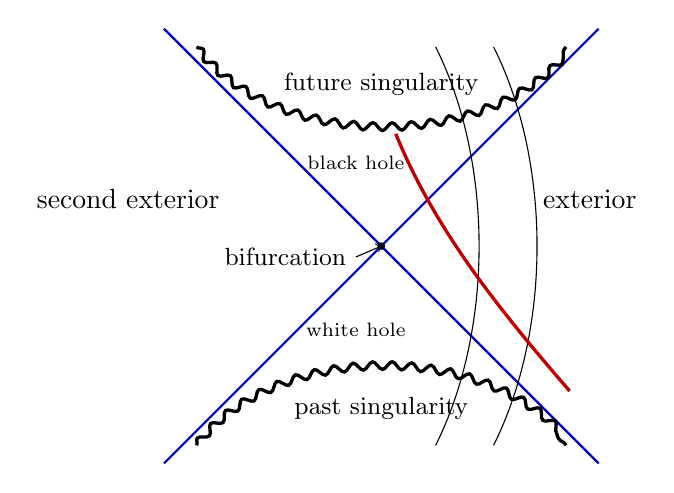
\begin{tikzpicture}[scale=0.92]
\draw[blue!75!black,thick] (-3,-3) -- (3,3);
\draw[blue!75!black,thick] (-3,3) -- (3,-3);
\draw[very thick,decorate,decoration={snake,amplitude=1.4pt,segment length=7pt}]
  (-2.55,2.75) .. controls (-1.45,1.35) and (1.45,1.35) .. (2.55,2.75);
\draw[very thick,decorate,decoration={snake,amplitude=1.4pt,segment length=7pt}]
  (-2.55,-2.75) .. controls (-1.45,-1.35) and (1.45,-1.35) .. (2.55,-2.75);
\draw (0.75,-2.75) .. controls (1.55,-1.15) and (1.55,1.15) .. (0.75,2.75);
\draw (1.55,-2.75) .. controls (2.35,-1.15) and (2.35,1.15) .. (1.55,2.75);
\draw[red!75!black,very thick] (2.6,-2.0) .. controls (1.65,-0.9) and (0.75,0.2) .. (0.2,1.55);
\fill (0,0) circle (1.5pt);
\node[above,font=\small] at (0,1.95) {future singularity};
\node[below,font=\small] at (0,-1.95) {past singularity};
\node[right] at (2.10,0.65) {exterior};
\node[left] at (-2.10,0.65) {second exterior};
\node[font=\scriptsize] at (-0.35,1.15) {black hole};
\node[font=\scriptsize] at (-0.35,-1.15) {white hole};
\node[font=\small,anchor=east] (bifurcation-label) at (-0.35,-0.15) {bifurcation};
\draw[->,thin] (bifurcation-label.east) -- (0,0);
\end{tikzpicture}
\caption{Một bức tranh nhân quả chưa compact hóa đã được làm gọn. Các chân trời null cắt nhau tại mặt phân nhánh; các điểm kỳ dị kiểu không gian nằm trong các nêm tương lai và quá khứ.}
\end{figure}

\subsection{Điều có thể xảy ra không phải là điều điển hình}

Cơ học vi mô bất biến dưới phép đảo ngược thời gian với độ chính xác rất cao, nhưng các lịch sử vĩ mô lại có một chiều ưu tiên. Một quả bom dễ dàng phát nổ; các mảnh văng ra hầu như không bao giờ tụ lại để dựng nó trở lại. Một quả bóng dễ dàng lăn xuống từ một đỉnh không ổn định; một quả bóng bị ném ngẫu nhiên hầu như không bao giờ dừng lại chính xác ở đó. Một tam giác bi-a đã được xếp sẵn dễ dàng tán xạ, trong khi các quả bi tán xạ không tự phát sắp xếp thành thế xếp đó. Một cục nước đá tan trong nước nóng, còn nước hầu như không bao giờ đẩy ra một cục nước đá mới được lắp ghép.

Sự khác biệt nằm ở entropy. Một trạng thái vĩ mô entropy thấp chiếm một vùng rất nhỏ của không gian pha; một trạng thái vĩ mô entropy cao chứa một số lượng khổng lồ các cách sắp xếp vi mô. Các phương trình cho phép quỹ đạo đảo ngược, nhưng việc chuẩn bị vi trạng thái ban đầu của nó đòi hỏi những tương quan chính xác đến mức phi thường.

\begin{classroomqa}
\audiencequestion{Chẳng phải mỗi cấu hình tán xạ chính xác đều hiếm chẳng kém cấu hình đảo thời gian chính xác sao?\lecturetimestamp{00:56:55}}
\lecturerresponse{Đúng, đối với các vi trạng thái được chỉ định riêng lẻ. Sự bất đối xứng xuất hiện khi ta so sánh các trạng thái vĩ mô. Một cách sắp xếp tán xạ bao gồm nhiều vi trạng thái hơn rất nhiều so với một tam giác được xếp chính xác, nên gần như mọi trạng thái vi mô tương thích với mô tả thứ nhất vẫn hỗn độn ở mức vĩ mô.}
\end{classroomqa}

Một lỗ trắng phát ra một Alice được tổ chức hoàn chỉnh là phiên bản hấp dẫn của một lịch sử làm giảm entropy như vậy. Nó được các phương trình thuận nghịch cho phép nhưng đòi hỏi một quá khứ đặc biệt đến mức khác thường. Bản thân chân trời mang entropy và thông tin vi mô bị che giấu, nên một dao động cỡ Alice không bị cấm về mặt logic; nó bị áp chế một cách áp đảo.

\begin{classroomqa}
\audiencequestion{Một dao động như vậy sẽ là lượng tử hay nhiệt?\lecturetimestamp{00:59:48}}
\lecturerresponse{Cả hai loại đều có thể đóng góp. Trong một hệ nóng thông thường, ngôn ngữ chi phối là dao động nhiệt; đối với lỗ đen, các hiệu ứng lượng tử và nhiệt đan xen vào nhau. Dù theo cách nào, sự áp chế trung tâm vẫn là entropic.}
\end{classroomqa}

\section{Khoảng cách riêng và phép compact hóa Penrose}

Trước khi vẽ không-thời gian toàn cục, ta nên làm cho thuật ngữ hướng tâm trở nên chính xác. Thời gian riêng là cái mà một chiếc đồng hồ đo dọc theo một đường thế giới kiểu thời gian. Khoảng cách riêng là cái mà một chuỗi thước mét cục bộ đo dọc theo một đường cong kiểu không gian đã chọn. Đối với lát Schwarzschild có \(t\) không đổi,
\begin{equation}
d\rho=\frac{dr}{\sqrt{1-2GM/r}}.
\label{eq:l04-proper-distance}
\end{equation}
Vì vậy \(r\) là một tọa độ diện tích, chứ không phải khoảng cách thước đo trực tiếp tính từ chân trời.

Bây giờ hãy bắt đầu với không-thời gian phẳng theo phương hướng tâm. Chỉ giữ lại \(t\) và \(\rho\ge0\). Đường \(\rho=0\) là gốc không gian, và một tia sáng hướng tâm đi vào gốc sẽ tiếp tục đi ra ngoài ở phía vật lý đối diện, điều này hiện ra như một phép phản xạ trong nửa mặt phẳng đã rút gọn.

Một sơ đồ Penrose ánh xạ mọi giá trị hữu hạn và vô hạn của \(t\) và \(\rho\) vào một miền hữu hạn trong khi bảo toàn các hướng null. Hai quy tắc của nó là:
\begin{enumerate}
\item compact hóa toàn bộ không-thời gian vào một miền hữu hạn;
\item giữ các tia sáng hướng tâm ở \(45^\circ\).
\end{enumerate}
Độ dài và các góc thông thường bị biến dạng; các quan hệ nhân quả thì không.

\begin{figure}[htbp]
\centering
\includegraphics[width=0.70\textwidth]{lecture_04_figure_06.png}
\caption{Lưới compact hóa hoàn chỉnh cho không-thời gian Minkowski hướng tâm. Thời gian vô hạn nằm tại các đầu mút trên và dưới bên trái, còn bán kính vô hạn bị nén vào đỉnh bên phải.}
\lectureframe{01:14:44.040}
\end{figure}

\begin{figure}[htbp]
\centering
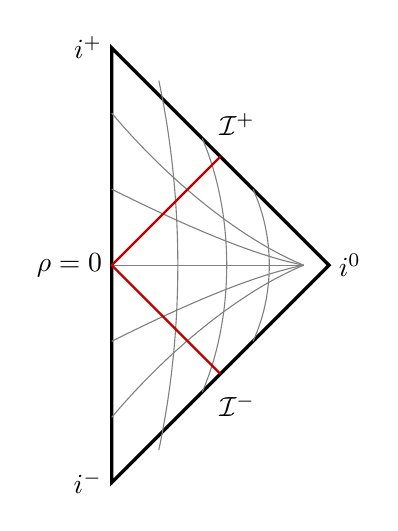
\begin{tikzpicture}[scale=0.92]
\coordinate (im) at (0,-3);
\coordinate (ip) at (0,3);
\coordinate (iz) at (3,0);
\draw[very thick] (im) -- (ip) -- (iz) -- cycle;
\draw[gray] (0,-2.1) .. controls (0.8,-1.15) and (1.8,-0.35) .. (2.65,0);
\draw[gray] (0,-1.05) .. controls (0.9,-0.6) and (1.9,-0.15) .. (2.65,0);
\draw[gray] (0,0) -- (2.65,0);
\draw[gray] (0,1.05) .. controls (0.9,0.6) and (1.9,0.15) .. (2.65,0);
\draw[gray] (0,2.1) .. controls (0.8,1.15) and (1.8,0.35) .. (2.65,0);
\draw[gray] (0.65,-2.55) .. controls (1.0,-0.9) and (1.0,0.9) .. (0.65,2.55);
\draw[gray] (1.25,-1.75) .. controls (1.7,-0.7) and (1.7,0.7) .. (1.25,1.75);
\draw[gray] (1.95,-1.05) .. controls (2.25,-0.4) and (2.25,0.4) .. (1.95,1.05);
\draw[red!75!black,thick] (1.5,-1.5) -- (0,0) -- (1.5,1.5);
\node[left] at (ip) {\(i^+\)};
\node[left] at (im) {\(i^-\)};
\node[right] at (iz) {\(i^0\)};
\node[above right] at (1.35,1.65) {\(\mathcal{I}^+\)};
\node[below right] at (1.35,-1.65) {\(\mathcal{I}^-\)};
\node[left] at (0,0) {\(\rho=0\)};
\end{tikzpicture}
\caption{Không-thời gian Minkowski hướng tâm trong một tam giác hữu hạn. Tia null màu đỏ đi vào từ \(\mathcal{I}^-\), đến gốc, và đi ra qua \(\mathcal{I}^+\).}
\label{fig:l04-flat-penrose}
\end{figure}

Các điểm mút có những ý nghĩa nhân quả khác nhau:
\begin{equation}
\begin{aligned}
i^-&:\ \text{past timelike infinity},\\
i^+&:\ \text{future timelike infinity},\\
i^0&:\ \text{spatial infinity},\\
\mathcal{I}^-&:\ \text{past null infinity},\\
\mathcal{I}^+&:\ \text{future null infinity}.
\end{aligned}
\end{equation}
Các ký hiệu \(\mathcal{I}^{-}\) và \(\mathcal{I}^{+}\) được đọc là scri minus và scri plus.

\begin{classroomqa}
\audiencequestion{Một tia null có nên đi qua các góc của mọi ô lưới bị biến dạng, và do đó hơi cong đi không?\lecturetimestamp{01:11:08}}
\lecturerresponse{Nếu toàn bộ lưới tọa độ được vẽ chính xác, các giao điểm của nó sẽ phù hợp với đường cong null. Phép dựng cốt yếu là bảo giác: các hướng null hướng tâm vẫn ở \(45^\circ\), mặc dù các đường lưới \(t\) không đổi và \(\rho\) không đổi bị uốn cong và dồn lại.}
\end{classroomqa}

\begin{classroomqa}
\audiencequestion{Nếu một tia sáng không đi qua gốc thì nó được vẽ như thế nào?\lecturetimestamp{01:11:45}}
\lecturerresponse{Nó đạt tới một khoảng cách tiếp cận gần nhất khác không rồi quay ra ngoài. Khi còn giữ chuyển động góc, hình chiếu hướng tâm của nó không nhất thiết là một đường thẳng \(45^\circ\) duy nhất.}
\end{classroomqa}

\begin{classroomqa}
\audiencequestion{Vậy tại sao tia sáng đó không ở \(45^\circ\)?\lecturetimestamp{01:12:49}}
\lecturerresponse{Quy tắc \(45^\circ\) được phát biểu cho các tia sáng hướng tâm. Một tia null mang mômen góc dành một phần chuyển động của nó cho các hướng góc, nên hình chiếu của nó lên mặt phẳng \(t\)-\(\rho\) không phải là hướng tâm.}
\end{classroomqa}

\section{Sơ đồ Schwarzschild vĩnh cửu}

Sơ đồ đã compact hóa có bốn miền. Hai hình thoi ở hai bên của nó là các miền bên ngoài phẳng tiệm cận. Tam giác phía trên là nội vùng lỗ đen và kết thúc tại điểm kỳ dị kiểu không gian trong tương lai. Tam giác phía dưới là miền lỗ trắng và bắt đầu tại điểm kỳ dị kiểu không gian trong quá khứ. Hợp lại, các miền này tạo thành hình học Schwarzschild mở rộng tối đại.

\begin{figure}[htbp]
\centering
\includegraphics[width=0.74\textwidth]{lecture_04_figure_07.png}
\caption{Sơ đồ Penrose Schwarzschild vĩnh cửu hoàn chỉnh, với các điểm kỳ dị, các chân trời, các quỹ đạo null và một biên tiệm cận được đánh dấu trên bảng.}
\lectureframe{01:21:30.000}
\end{figure}

\begin{figure}[htbp]
\centering
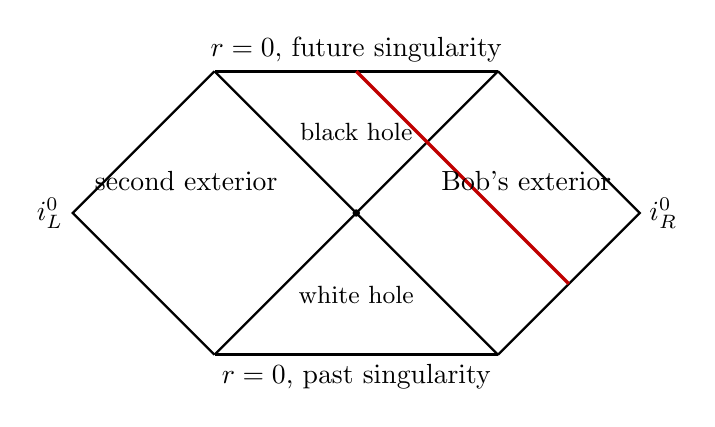
\begin{tikzpicture}[scale=0.90]
\coordinate (C) at (0,0);
\coordinate (TL) at (-2,2);
\coordinate (TR) at (2,2);
\coordinate (BL) at (-2,-2);
\coordinate (BR) at (2,-2);
\coordinate (L) at (-4.0,0);
\coordinate (R) at (4.0,0);
\draw[very thick] (TL) -- (TR);
\draw[very thick] (BL) -- (BR);
\draw[thick] (C) -- (TL) (C) -- (TR) (C) -- (BL) (C) -- (BR);
\draw[thick] (TL) -- (L) -- (BL);
\draw[thick] (TR) -- (R) -- (BR);
\draw[red!75!black,very thick] (3,-1) -- (1,1) -- (0,2);
\node[above] at (0,2) {\(r=0\), future singularity};
\node[below] at (0,-2) {\(r=0\), past singularity};
\node[font=\small] at (0,1.15) {black hole};
\node[font=\small] at (0,-1.15) {white hole};
\node at (2.4,0.45) {Bob's exterior};
\node at (-2.4,0.45) {second exterior};
\node[right] at (R) {\(i^0_R\)};
\node[left] at (L) {\(i^0_L\)};
\fill (C) circle (1.5pt);
\end{tikzpicture}
\caption{Bốn miền của Schwarzschild vĩnh cửu. Một tia sáng hướng tâm đi vào cắt qua chân trời tương lai và kết thúc tại \(r=0\).}
\label{fig:l04-eternal}
\end{figure}

Một tia sáng hướng tâm đi vào từ \(\mathcal{I}^-\) cắt qua chân trời tương lai và kết thúc ở điểm kỳ dị. Mọi đường cong nhân quả trong tam giác phía trên đều chung số phận đó. Miền bên ngoài thứ hai thường được mô tả là miệng kia của một cầu Einstein--Rosen, nhưng nó không thể đi xuyên qua: bất kỳ chuyến đi nhân quả nào được thử từ một miền bên ngoài sang miền kia đều đi vào vùng lỗ đen và chạm tới điểm kỳ dị.

\begin{classroomqa}
\audiencequestion{Hai thế giới bên ngoài có được nối với nhau bằng một hố sâu, và có thể gửi tín hiệu qua đó không?\lecturetimestamp{01:22:21}}
\lecturerresponse{Hình học vĩnh cửu chứa một cầu Einstein--Rosen trên các lát không gian thích hợp, nhưng không có tín hiệu nhân quả nào đi từ miền bên ngoài này sang miền bên ngoài kia. Cầu đó thắt lại quá nhanh; ngay cả ánh sáng đi vào một chân trời cũng kết thúc ở điểm kỳ dị tương lai.}
\end{classroomqa}

Sơ đồ này mô tả một lỗ đã tồn tại từ mọi thời. Các lỗ vật lý thiên văn thực sự được hình thành từ vật chất suy sụp. Sơ đồ nhân quả của chúng không có điểm kỳ dị lỗ trắng trong quá khứ và không có miền bên ngoài phẳng tiệm cận thứ hai. Để xây dựng hình học đó, ta cần hiểu các vỏ cầu.

\section{Tạo ra một lỗ đen bằng sự suy sụp}

Hãy hình dung một vỏ cầu loãng gồm các hạt đi vào. Chúng có thể là photon: năng lượng gây hấp dẫn, nên một xung bức xạ đủ tập trung có thể tạo thành một lỗ đen. Trước khi suy sụp, miền trung tâm giống không-thời gian phẳng rỗng; sau khi đủ năng lượng bị nén lại, miền bên ngoài giống Schwarzschild. Nhiệm vụ là ghép các miền đó qua vỏ đang chuyển động.

\subsection{Định lý vỏ cầu của Newton}

Đối với một vỏ cầu Newton đối xứng cầu có tổng khối lượng \(M\), định luật Gauss cho hấp dẫn có dạng
\begin{equation}
\oint \mathbf{g}\cdot d\mathbf{A}=-4\pi G M_{\mathrm{enc}}.
\label{eq:l04-gauss-gravity}
\end{equation}
Đối xứng cầu khiến \(\mathbf{g}=g(r)\hat{\mathbf r}\), nên
\begin{equation}
g(r)=
\begin{cases}
0, & r<R_{\mathrm{shell}},\\[4pt]
-\dfrac{GM}{r^2}, & r>R_{\mathrm{shell}}.
\end{cases}
\label{eq:l04-shell-field}
\end{equation}
Ở bên trong, không có khối lượng nào được bao kín và trường hấp dẫn triệt tiêu. Ở bên ngoài, vỏ tác dụng đúng hệt như một khối lượng điểm \(M\) tại tâm. Thế hấp dẫn bên trong là hằng số chứ không phải bằng 0, nhưng không còn lực Newton cục bộ nào.\editorialnote{Lập luận bằng các đường sức được đưa ra trong lớp học được định luật Gauss mô tả một cách chính xác. Sự khác biệt giữa trường bằng 0 và thế hằng số là quan trọng khi so sánh các chuẩn hóa đồng hồ trong thuyết tương đối.}

Kết luận ấy vẫn đúng khi một vỏ cầu hoàn toàn đối xứng cầu co lại, miễn là tổng khối lượng của nó được bảo toàn. Chỉ vị trí của biên giữa nghiệm bên trong và nghiệm bên ngoài thay đổi.

\subsection{Định lý Birkhoff}

Đối ứng tương đối tính của nó là định lý Birkhoff: mọi miền chân không đối xứng cầu đều cục bộ là một phần của họ Schwarzschild. Với một vỏ không có khối lượng ở tâm,
\begin{align}
ds^2_{\mathrm{inside}}&=-dT^2+dR^2+R^2d\Omega_2^2,\\
ds^2_{\mathrm{outside}}&=
-\left(1-\frac{2GM}{r}\right)dt^2
\nonumber\\
&\quad+\frac{dr^2}{1-2GM/r}
+r^2d\Omega_2^2.
\label{eq:l04-birkhoff-pieces}
\end{align}

\begin{figure}[htbp]
\centering
\includegraphics[width=0.74\textwidth]{lecture_04_figure_08.png}
\caption{Bảng ghép vỏ: không-thời gian phẳng ở bên trong đường tròn và nghiệm Schwarzschild ở bên ngoài.}
\lectureframe{01:34:15.000}
\end{figure}

\begin{classroomqa}
\audiencequestion{Metric nào xuất hiện bên ngoài một vỏ cầu trong thuyết tương đối rộng?\lecturetimestamp{01:33:17}}
\lecturerresponse{Metric Schwarzschild, với tham số khối lượng bằng tổng khối lượng bảo toàn của vỏ. Miền trung tâm rỗng là không-thời gian Minkowski cục bộ.}
\end{classroomqa}

\begin{classroomqa}
\audiencequestion{Nếu vỏ co lại, tại sao tham số khối lượng không thay đổi?\lecturetimestamp{01:34:33}}
\lecturerresponse{Vì tổng năng lượng được bảo toàn. Bán kính của vỏ và các đóng góp động năng hoặc năng lượng liên kết của nó có thể thay đổi, nhưng khối lượng bên ngoài được bảo toàn là cố định đối với một hệ cầu cô lập. Vỏ chuyển động làm thay đổi nơi mà các miền phẳng và Schwarzschild được ghép lại.}
\end{classroomqa}

Miền trong phẳng không có nghĩa là một đồng hồ ở bên trong tất yếu có cùng chuẩn hóa như một đồng hồ ở vô cực. Việc ghép qua vỏ có thể nhân tọa độ thời gian bên trong với một hằng số, và một vỏ chuyển động đòi hỏi các điều kiện nối tương ứng.\editorialnote{Định lý Birkhoff xác định cục bộ từng vùng chân không. Quan hệ toàn cục giữa các tọa độ của chúng được xác định bằng cách ghép metric cảm sinh và độ cong ngoại lai qua vỏ. Các chi tiết đó được để lại sau, đúng như cách phép dựng sự sụp đổ được để lại cho bài giảng tiếp theo.}

Giờ đây ta đã có hai mảnh cần thiết cho sự hình thành: không-thời gian Minkowski ở bên trong vỏ co lại và không-thời gian Schwarzschild ở bên ngoài nó. Khi vỏ dịch vào trong, mặt phân cách giữa chúng vạch nên một ống thế giới. Theo dõi ống đó đi qua bán kính Schwarzschild giả định sẽ thay thế nửa quá khứ phi vật lý của Hình~\ref{fig:l04-eternal} bằng một vùng tiền sụp đổ chính quy và cho thấy chân trời sự kiện của một lỗ đen thực sự bắt đầu ở đâu.
